\section{8th sheaf cobordism}
Suppose we have a punctured Riemann sphere $M$ and $\Lambda_0^0$, $\Lambda_0^\infty$, $\Lambda_0^{squig}$, a nested regions $U\subset U' \subset M$, and a chart $f : U \rightarrow \R^2$ such that $U'$ maps to $R:=(-2,2)_x \times (-1,1)_z$ under $f$
\begin{itemize}
\item $\Lambda_0^0$ gets mapped to blue strands in the below figure, co-oriented upward.

\item $\Lambda_0^\infty$ gets mapped to red strands in the below figure, co-oriented downward.

\item $\Lambda_0^{squig}$ gets mapped to squiggly lines with co-orientations given in the figure below.
\end{itemize}
and a sheaf defined by the following squiggly legible diagram. All the maps corresponding to blue strands are $\iota_1$ and the red strands $\iota_0$ otherwise stated. I have omitted these maps from the diagram.\\

\begin{figure}[H]
    \centering
    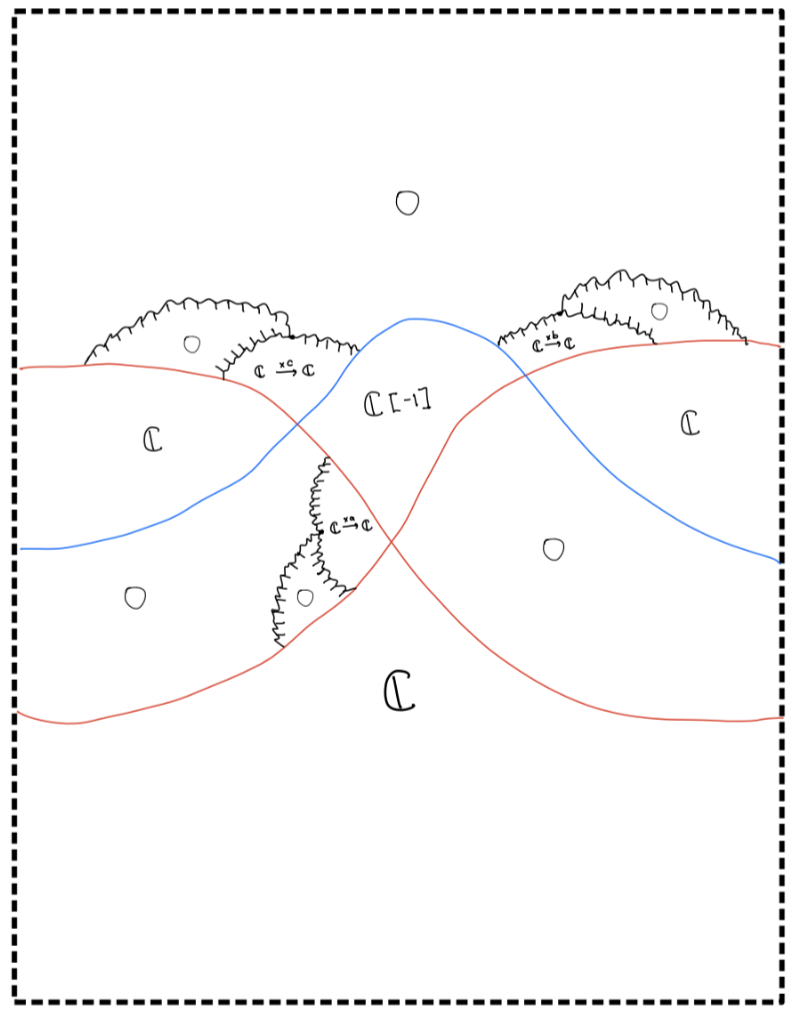
\includegraphics[scale = 0.85]{diagrams/cobord8/1.png}
    \caption{}
    \label{fig:your-label}
\end{figure}

Then we define a cobordism starting from the above sheaf, say $cobord_8$ supported on $U$. At the end of the cobordism, the sheaf, under the same chart $f$, is described as the following squiggly legible diagram.

\begin{figure}[H]
    \centering
    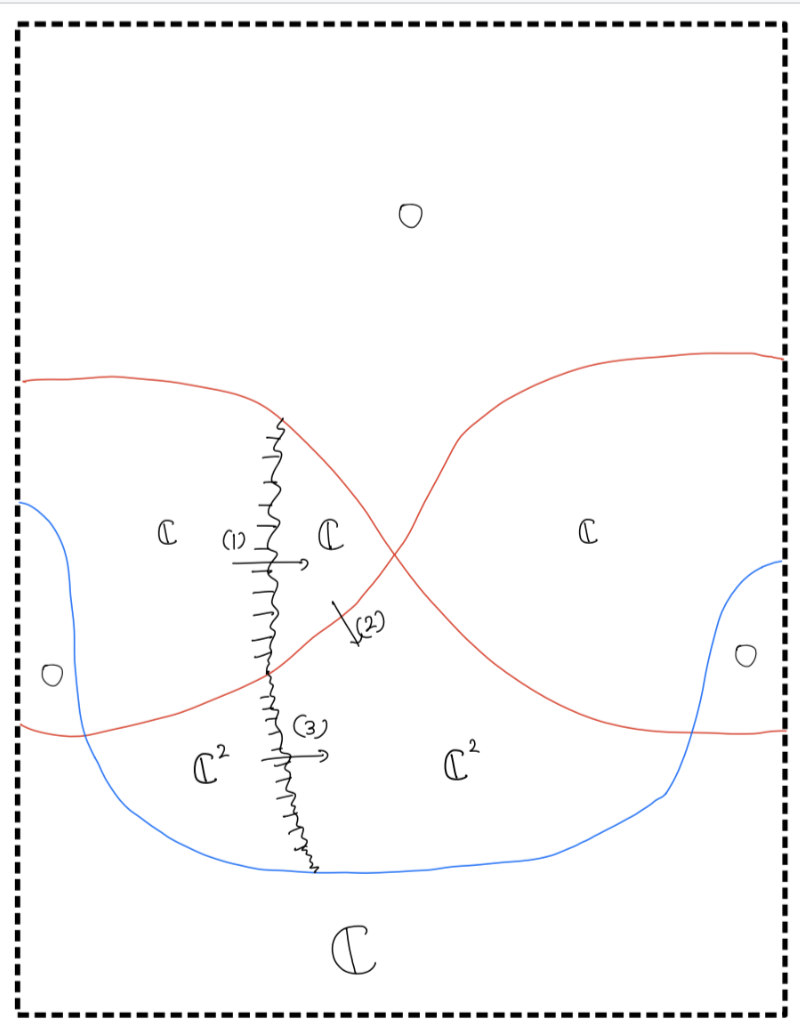
\includegraphics[scale = 0.85]{diagrams/cobord8/11.png}
    \caption{}
    \label{fig:your-label}
\end{figure}
\textbf{Generizations maps}:
\begin{enumerate}[label = (\arabic*)]
\item $\times b^{-1}c$
\item 
$\begin{pmatrix}
1\\
-a^{-1}b
\end{pmatrix}$

\item 
$\begin{pmatrix}
b^{-1}c & 0\\
-a^{-1}c & 1
\end{pmatrix}$
\end{enumerate}
\pagebreak
We define $cobord_8$ as follows.
\begin{enumerate}[label=(Step \arabic*)]
\item we apply $cobord_1$ to the square regions surrounded by purple dotted lines.

\begin{figure}[H]
    \centering
    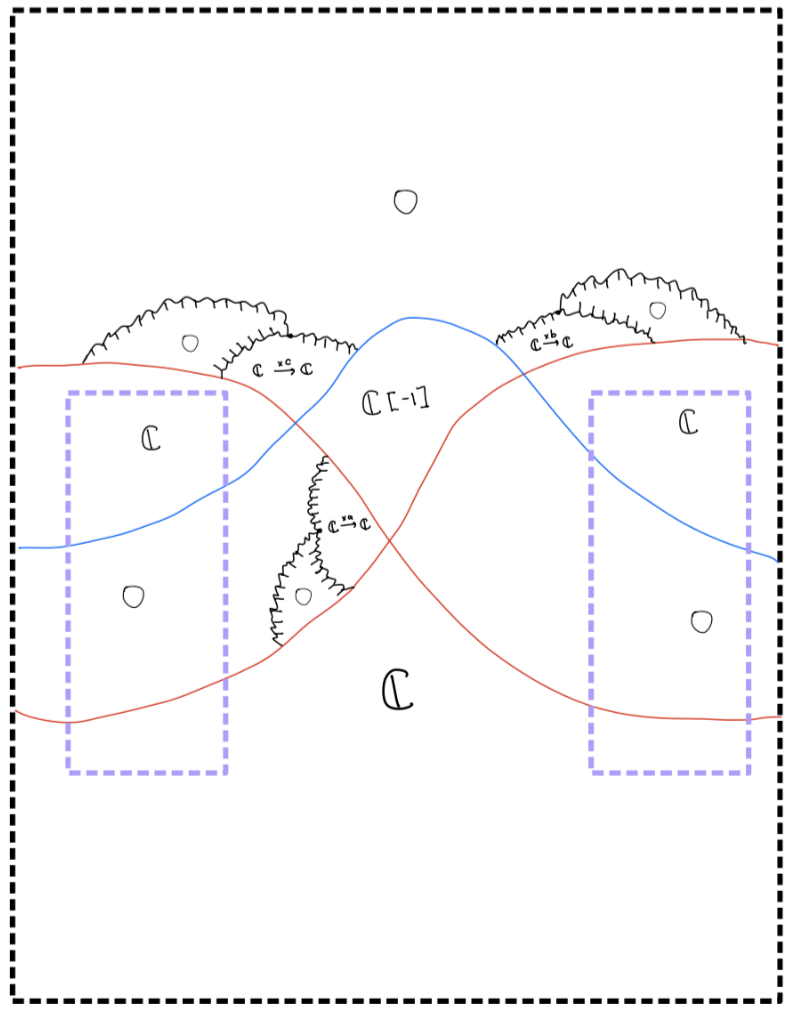
\includegraphics[scale = 0.85]{diagrams/cobord8/2.png}
    \caption{}
    \label{fig:your-label}
\end{figure}
\pagebreak
we get

\begin{figure}[H]
    \centering
    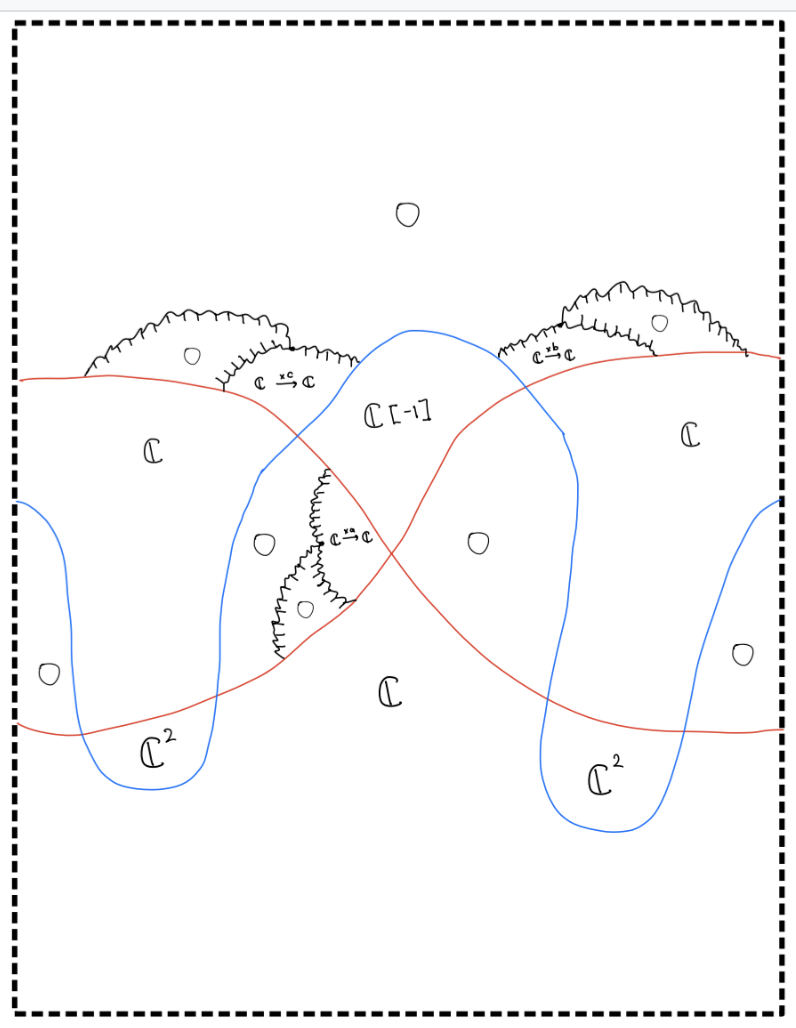
\includegraphics[scale = 0.85]{diagrams/cobord8/3.png}
    \caption{}
    \label{fig:your-label}
\end{figure}
\pagebreak
\item apply $cobord_4$ to the region surrounded by a purple dotted line.

\begin{figure}[H]
    \centering
    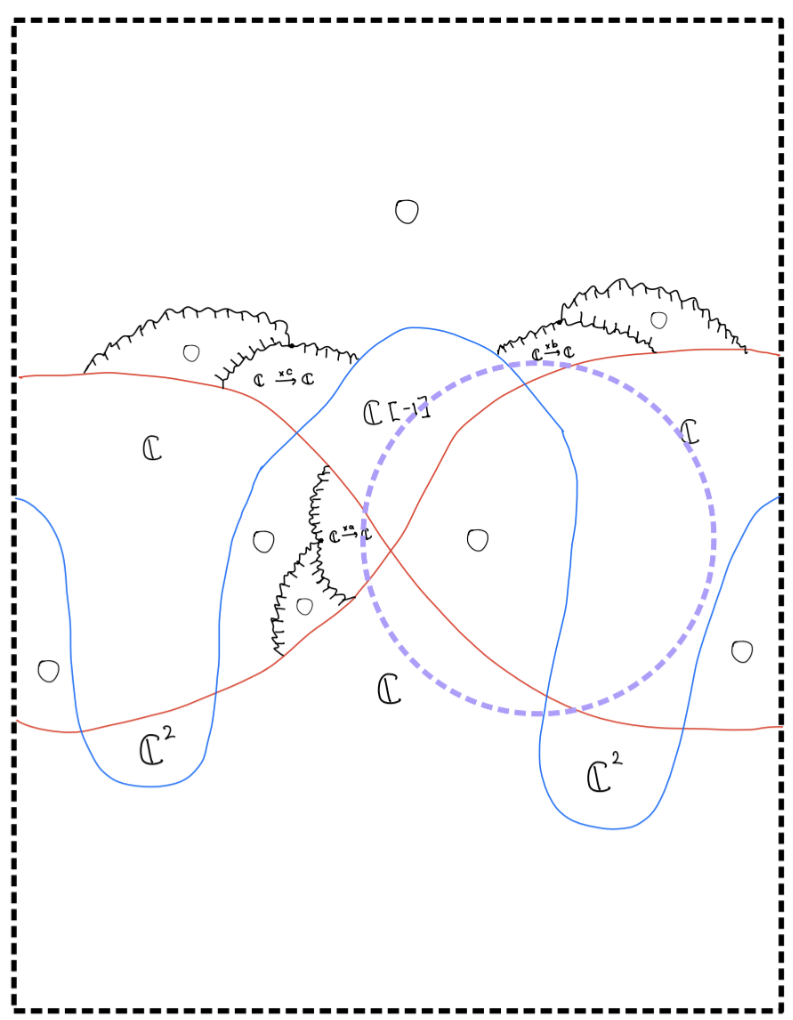
\includegraphics[scale = 0.85]{diagrams/cobord8/4.png}
    \caption{}
    \label{fig:your-label}
\end{figure}
\pagebreak
we get

\begin{figure}[H]
    \centering
    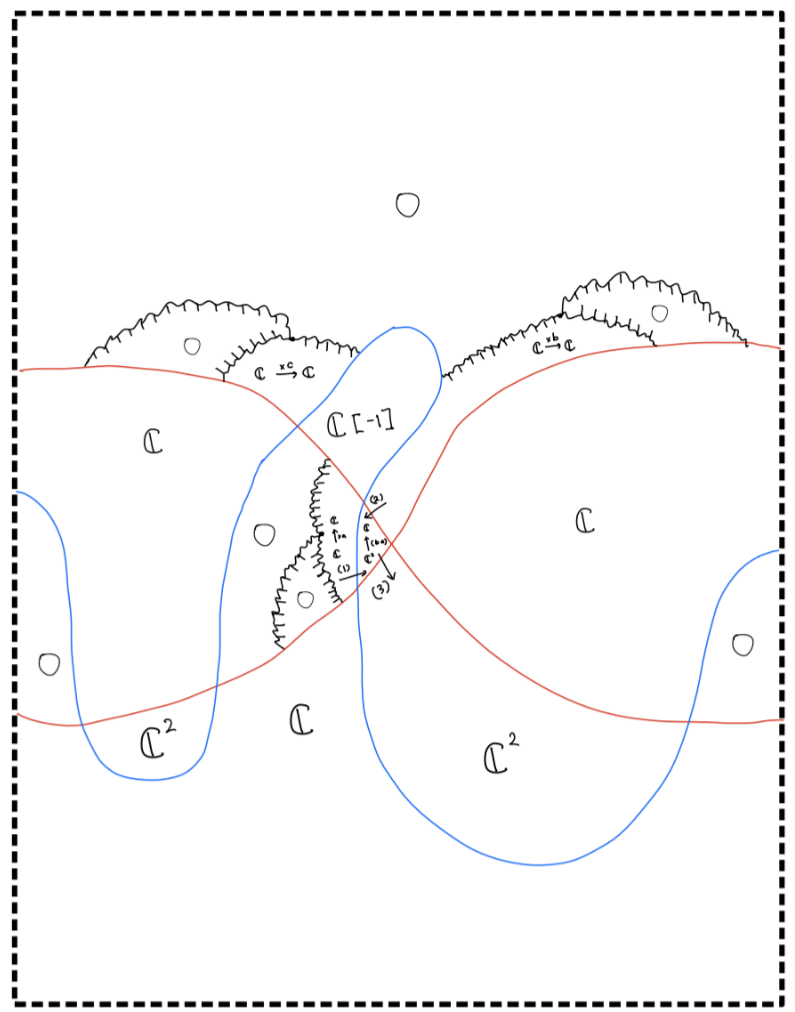
\includegraphics[scale = 1.15]{diagrams/cobord8/5.png}
    \caption{}
    \label{fig:your-label}
\end{figure}
\textbf{Generizations maps}:
\begin{enumerate}[label = (\arabic*)]
\item 
\begin{tikzcd}
\C \arrow[r, "\times 1"] & \C\\
\C \arrow[u,"\times a"]\arrow[r, "\iota_1"] & \C^2\arrow[u, "(b~a)"]
\end{tikzcd}

\item 
\begin{tikzcd}
\C \arrow[r, "\times 1"] & \C\\
\C \arrow[u,"\times b"]\arrow[r, "\iota_0"] & \C^2\arrow[u, "(b~a)"]
\end{tikzcd}

\item 
\begin{tikzcd}
\C \arrow[r] & 0 \\
\C^2 \arrow[u,"(b~a)"]\arrow[r, "id"] & \C^2\arrow[u]
\end{tikzcd}
\end{enumerate}
\pagebreak
\item apply $cobord'_2$ to the square region surrounded by purple dotted lines.

\begin{figure}[H]
    \centering
    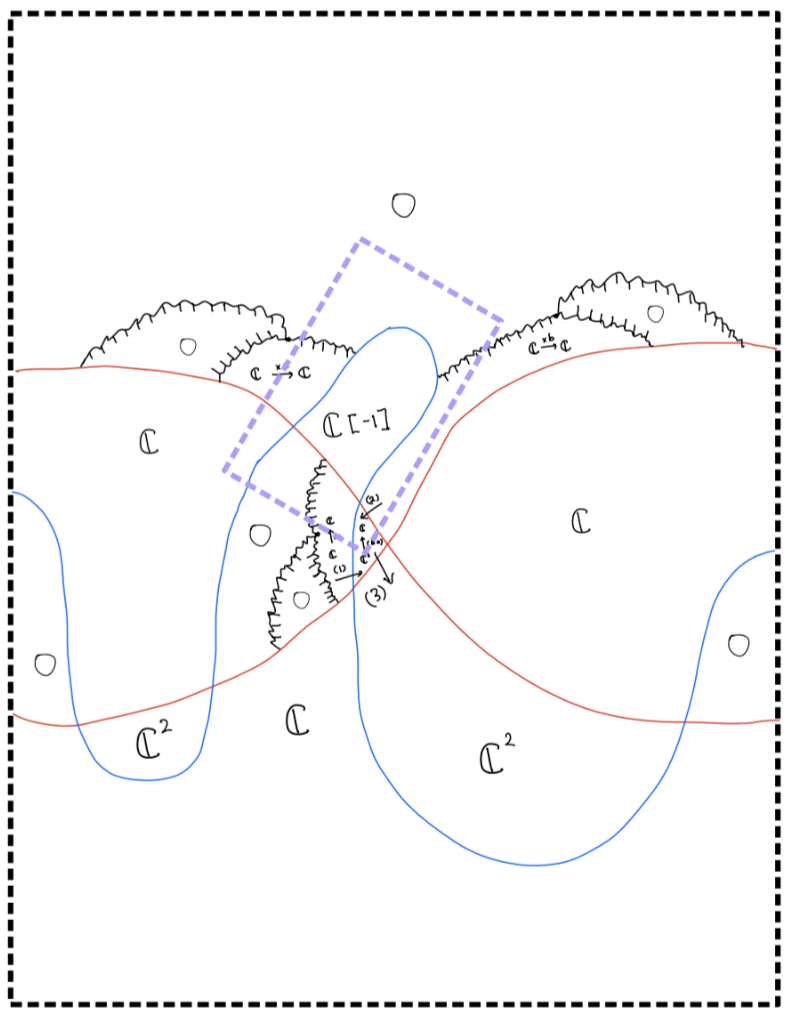
\includegraphics[scale = 0.85]{diagrams/cobord8/6.png}
    \caption{}
    \label{fig:your-label}
\end{figure}
\pagebreak
we get
\begin{figure}[H]
    \centering
    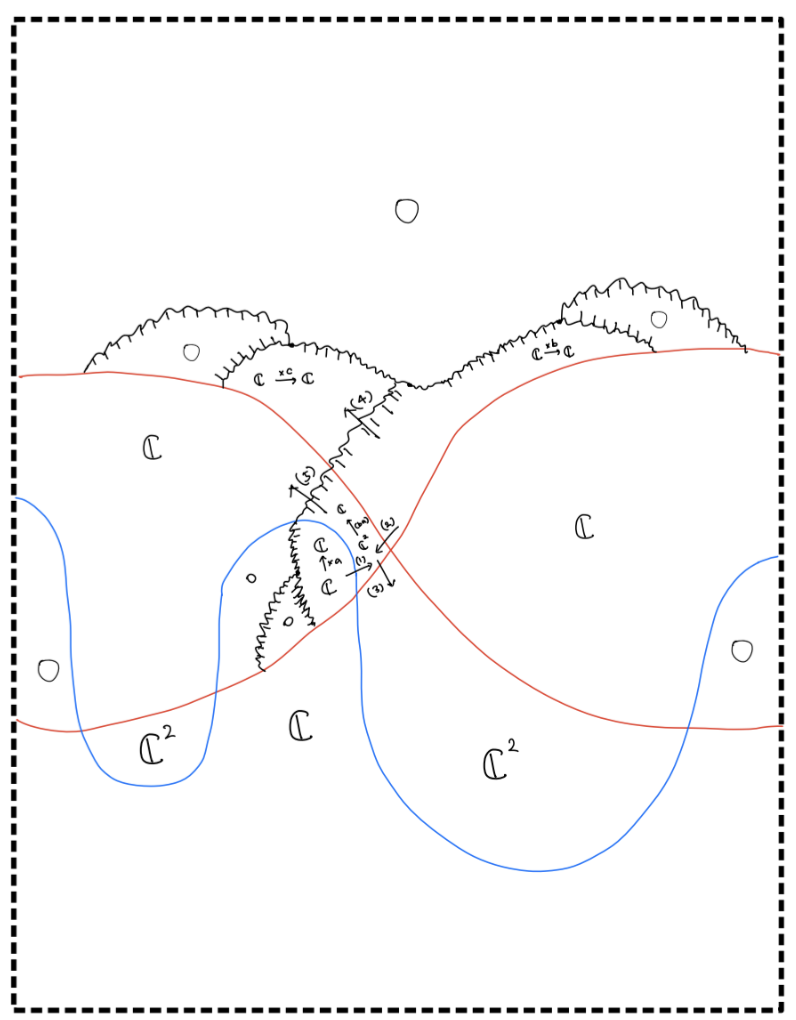
\includegraphics[scale = 1.1]{diagrams/cobord8/7.png}
    \caption{}
    \label{fig:your-label}
\end{figure}
\textbf{Generizations maps}:
\begin{enumerate}[label = (\arabic*)]
\item 
\begin{tikzcd}
\C \arrow[r, "\times 1"] & \C\\
\C \arrow[u,"\times a"]\arrow[r, "\iota_1"] & \C^2\arrow[u, "(b~a)"]
\end{tikzcd}

\item 
\begin{tikzcd}
\C \arrow[r, "\times 1"] & \C\\
\C \arrow[u,"\times b"]\arrow[r, "\iota_0"] & \C^2\arrow[u, "(b~a)"]
\end{tikzcd}

\item 
\begin{tikzcd}
\C \arrow[r] & 0 \\
\C^2 \arrow[u,"(b~a)"]\arrow[r, "id"] & \C^2\arrow[u]
\end{tikzcd}

\item 
\begin{tikzcd}
\C \arrow[r, "\times 1"] & \C\\
\C \arrow[u,"\times b"]\arrow[r, "\times bc^{-1}"] & \C\arrow[u, "c"]
\end{tikzcd}

\item 
\begin{tikzcd}
\C \arrow[r] & 0\\
\C \arrow[u,"(b~a)"]\arrow[r, "(bc^{-1} ~ 0)"] & \C\arrow[u]
\end{tikzcd}
\end{enumerate}
After identifying 
\begin{itemize}
\item $\C$ with $\C^2\xrightarrow{(b~a)} \C$ via
\begin{tikzcd}
\C \arrow[r] & 0\\
\C \arrow[u,"(b~a)"]\arrow[r, "(bc^{-1} ~ 0)"] & \C\arrow[u]
\end{tikzcd}

\item $\C\xrightarrow{\times a}\C$, $\C\xrightarrow{\times b}\C$, $\C\xrightarrow{\times c}\C$ with $0$
\end{itemize}
\pagebreak
the above sheaf is quasi-isomorphic to
\begin{figure}[H]
    \centering
    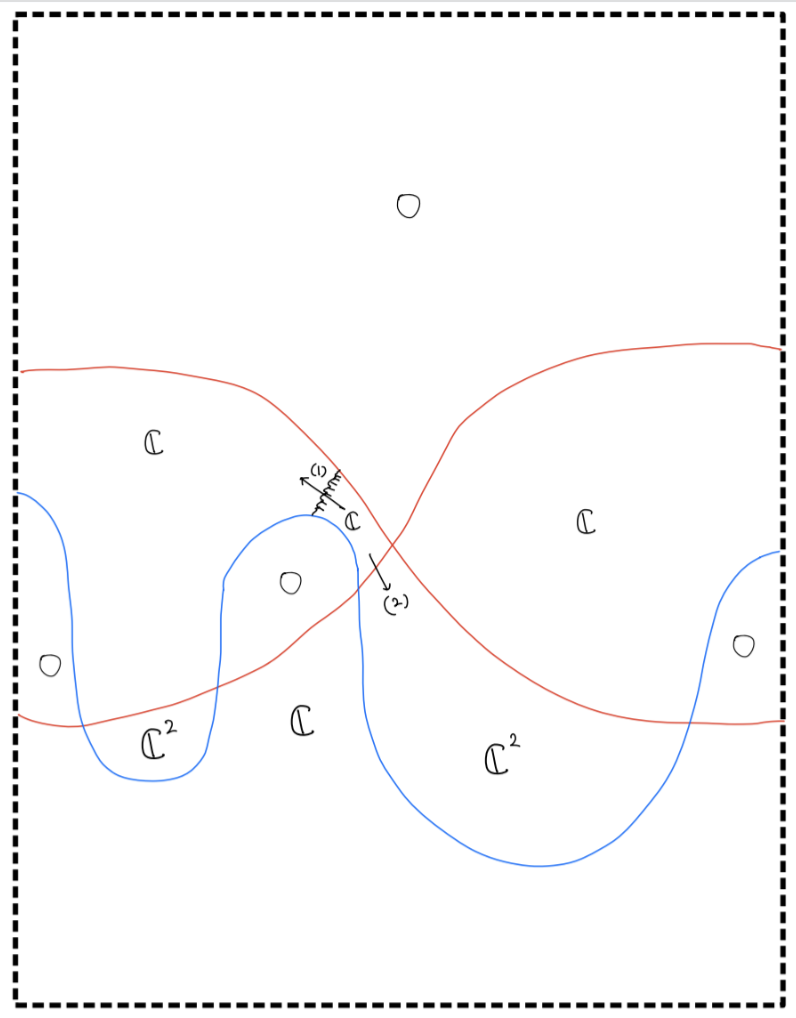
\includegraphics[scale = 0.85]{diagrams/cobord8/8.png}
    \caption{}
    \label{fig:your-label}
\end{figure}

\textbf{Generizations maps}:
\begin{enumerate}[label = (\arabic*)]
\item $\times bc^{-1}$
\item 
$\begin{pmatrix}
1\\
-a^{-1}b
\end{pmatrix}$
\end{enumerate}
\pagebreak
which is quasi-isomorphic to
\begin{figure}[H]
    \centering
    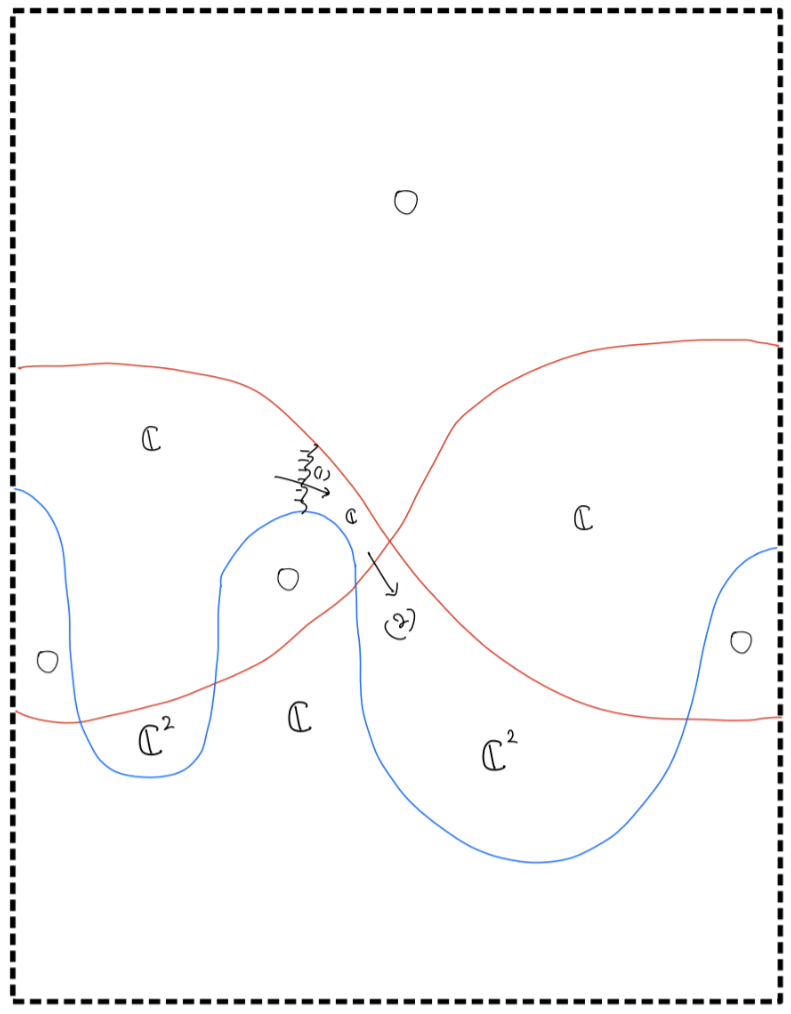
\includegraphics[scale = 0.85]{diagrams/cobord8/9.png}
    \caption{}
    \label{fig:your-label}
\end{figure}
\textbf{Generizations maps}:
\begin{enumerate}[label = (\arabic*)]
\item $\times b^{-1}c$
\item 
$\begin{pmatrix}
1\\
-a^{-1}b
\end{pmatrix}$
\end{enumerate}
\pagebreak
\item apply $cobord_3$ to the region surrounded by a purple dotted line

\begin{figure}[H]
    \centering
    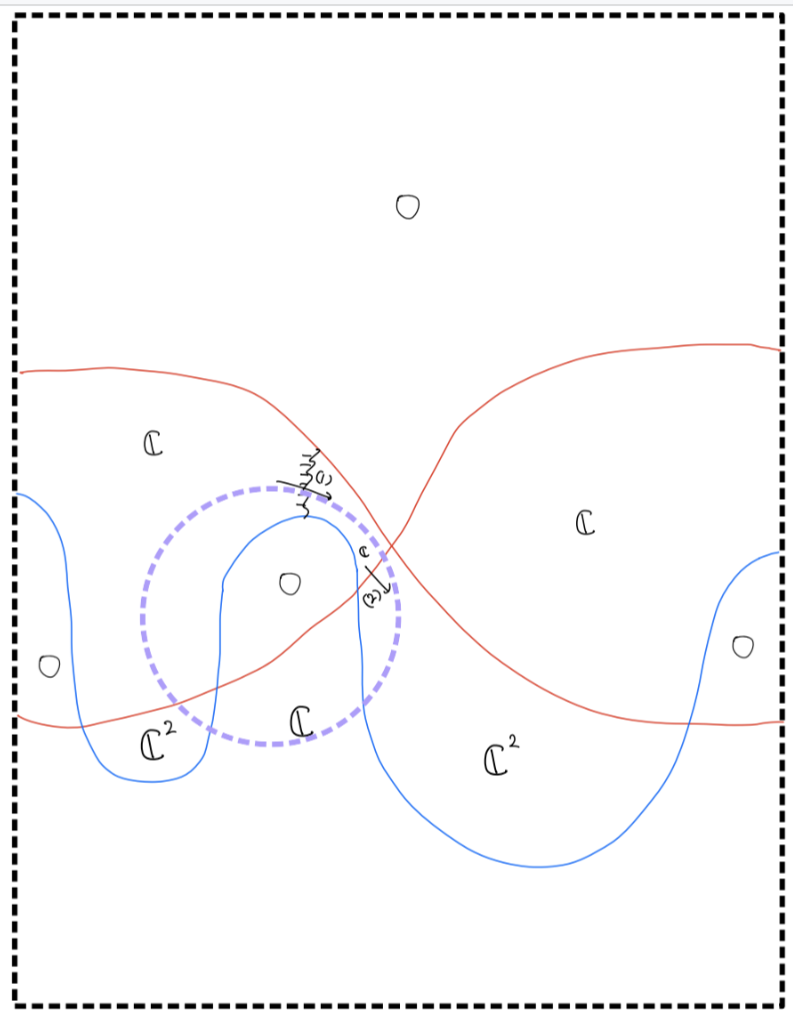
\includegraphics[scale = 0.85]{diagrams/cobord8/10.png}
    \caption{}
    \label{fig:your-label}
\end{figure}
\pagebreak
we get

\begin{figure}[H]
    \centering
    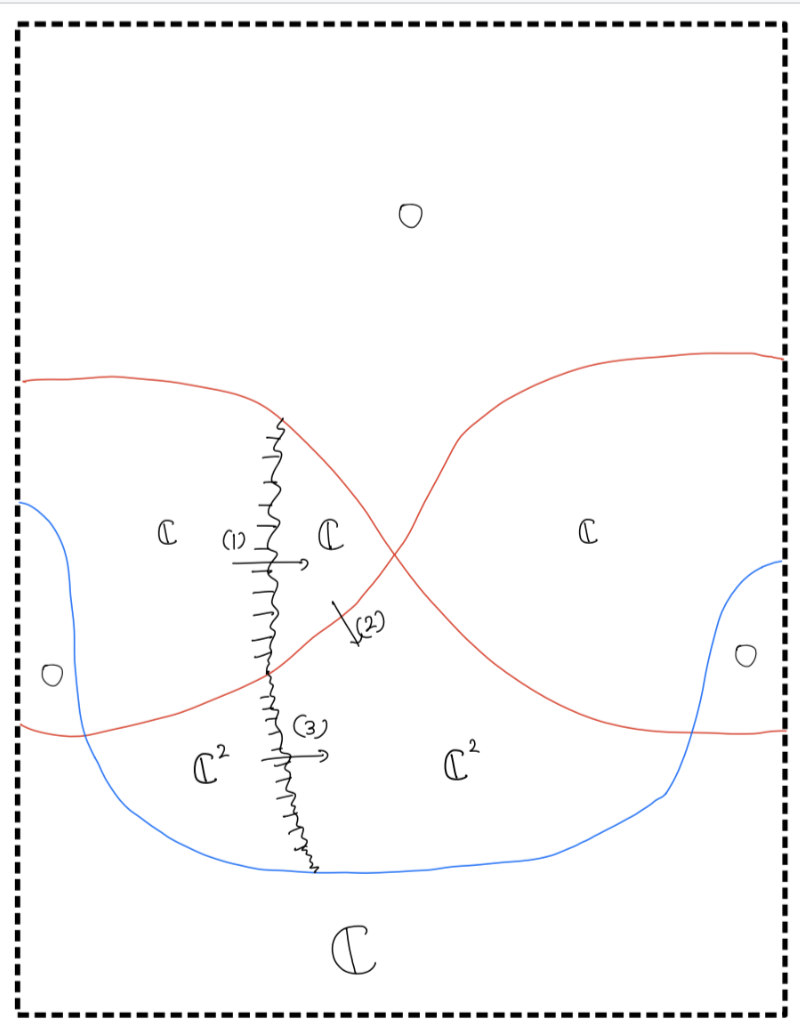
\includegraphics[scale = 0.8]{diagrams/cobord8/11.png}
    \caption{}
    \label{fig:your-label}
\end{figure}
\textbf{Generizations maps}:
\begin{enumerate}[label = (\arabic*)]
\item $\times b^{-1}c$
\item 
$\begin{pmatrix}
1\\
-a^{-1}b
\end{pmatrix}$

\item 
$\begin{pmatrix}
b^{-1}c & 0\\
-a^{-1}c & 1
\end{pmatrix}$
\end{enumerate}
\end{enumerate}
\pagebreak